\documentclass[12pt,]{article}
\usepackage[left=1in,top=1in,right=1in,bottom=1in]{geometry}
\newcommand*{\authorfont}{\fontfamily{bch}\selectfont}
\usepackage{lmodern}
\usepackage{abstract}
\renewcommand{\abstractname}{}    % clear the title
\renewcommand{\absnamepos}{empty} % originally center

\renewenvironment{abstract}
 {{%
    \setlength{\leftmargin}{0mm}
    \setlength{\rightmargin}{\leftmargin}%
    \footnotesize
  }%
  \relax}
 {\endlist}

\makeatletter
\def\@maketitle{%
  \newpage
%  \null
  \let \footnote \thanks
    {\fontsize{18}{20}\selectfont\centering  \setlength{\parindent}{0pt} \@title \par}%
  \vskip 2em%
}
%\fi
\makeatother




\setcounter{secnumdepth}{0}


\usepackage{graphicx}
% We will generate all images so they have a width \maxwidth. This means
% that they will get their normal width if they fit onto the page, but
% are scaled down if they would overflow the margins.
\makeatletter
\def\maxwidth{\ifdim\Gin@nat@width>\linewidth\linewidth
\else\Gin@nat@width\fi}
\makeatother
\let\Oldincludegraphics\includegraphics
\renewcommand{\includegraphics}[1]{\Oldincludegraphics[width=\maxwidth]{#1}}

\title{Does Media Coverage Drive Public Support for UKIP or Does Public Support
for UKIP Drive Media Coverage?\thanks{This is a draft working paper. Justin Murphy (\url{http://jmrphy.net})
is Assistant Professor of Politics at the University of Southampton.
Daniel Devine is a post-graduate researcher at the University of
Southampton. A previous version of this manuscript was presented at the
2016 annual meeting of the Political Studies Association in Brighton,
UK. Comments, questions, and suggestions are welcome and can be emailed
to \href{mailto:j.murphy@soton.ac.uk}{\nolinkurl{j.murphy@soton.ac.uk}}.
If you wish to cite, please use the citation and DOI provided with the
most up-to-date version of this manuscript, which will be maintained at
\url{http://j.mp/ukip-media}. This manuscript was last updated on April
22, 2016.}  }



\author{\Large Justin Murphy\vspace{0.05in} \newline\normalsize\emph{University of Southampton}   \and \Large Daniel Devine\vspace{0.05in} \newline\normalsize\emph{University of Southampton}  }


\date{}

\usepackage{titlesec}

\titleformat*{\section}{\normalsize\bfseries}
\titleformat*{\subsection}{\normalsize\itshape}
\titleformat*{\subsubsection}{\normalsize\itshape}
\titleformat*{\paragraph}{\normalsize\itshape}
\titleformat*{\subparagraph}{\normalsize\itshape}

\usepackage{natbib}
\bibliographystyle{plainnat}


\newtheorem{hypothesis}{Hypothesis}
\usepackage{setspace}

\makeatletter
\@ifpackageloaded{hyperref}{}{%
\ifxetex
  \usepackage[setpagesize=false, % page size defined by xetex
              unicode=false, % unicode breaks when used with xetex
              xetex]{hyperref}
\else
  \usepackage[unicode=true]{hyperref}
\fi
}
\@ifpackageloaded{color}{
    \PassOptionsToPackage{usenames,dvipsnames}{color}
}{%
    \usepackage[usenames,dvipsnames]{color}
}
\makeatother
\hypersetup{breaklinks=true,
            bookmarks=true,
            pdfauthor={Justin Murphy (University of Southampton) and Daniel Devine (University of Southampton)},
            pdfkeywords = {UKIP, media, public opinion, political parties, right-wing populism},  
            pdftitle={Does Media Coverage Drive Public Support for UKIP or Does Public Support
for UKIP Drive Media Coverage?},
            colorlinks=true,
            citecolor=BrickRed,
            urlcolor=MidnightBlue,
            linkcolor=MidnightBlue,
            pdfborder={0 0 0}}
\urlstyle{same}  % don't use monospace font for urls

\begin{document}  

% \maketitle

{% \usefont{T1}{pnc}{m}{n}
\setlength{\parindent}{0pt}
\thispagestyle{plain}
{\fontsize{18}{20}\selectfont\centering
\maketitle  % title \par  

}

{
   \relax \centering \normalsize\fontsize{11}{12} 
\textbf{\authorfont Justin Murphy} \\ \emph{\small University of Southampton} \\ \medskip  \par \textbf{\authorfont Daniel Devine} \\ \emph{\small University of Southampton} \\ \medskip 
  \vskip 1.5em%
}

}







\begin{abstract}

    \hbox{\vrule height .2pt width 39.14pc}

    \vskip 8.5pt % \small 

\noindent \footnotesize \textbf{Abstract:} Previous research suggests media attention may cause support for
populist right-wing parties, but extant evidence is mostly limited to
proportional representation systems in which such an effect would be
most likely. At the same time, in the United Kingdom's
first-past-the-post system, an ongoing political and regulatory debate
revolves around whether the media give disproportionate coverage to the
populist right-wing UK Independence Party (UKIP). We use a mixed-methods
research design to investigate the causal dynamics of UKIP support and
media coverage as an especially valuable case. Vector autoregression
(VAR) using monthly, aggregate time-series data from January 2004 to
February 2016 provides new evidence consistent with a model in which
media coverage drives party support, but not vice-versa. Additionally,
we identify key periods in which stagnating or declining support for
UKIP is followed by increases in media coverage and subsequent increases
in public support. The findings show that media coverage may drive
public support for right-wing populist parties, in a substantively
non-trivial fashion irreducible to previous levels of public support,
even in a national institutional environment least supportive of such an
effect. The findings have troubling implications for political debates
in the United Kingdom and potentially liberal democracies more
generally.


\vskip 8.5pt \noindent \footnotesize \emph{Keywords}: UKIP, media, public opinion, political parties, right-wing populism \par

    \hbox{\vrule height .2pt width 40pc}



\end{abstract}


\vskip 6.5pt

\noindent  \section{Introduction}\label{introduction}

If the visibility of a political party in the media shapes the public
support it receives, then the degree to which the media gives attention
to different political parties can have significant implications for
democracy. In the United Kingdom, critics allege that the media pays
disproportionate attention to the populist, right-wing UK Independence
Party (UKIP) but media elites claim that media coverage of UKIP is
driven by increasing public support for the party. Descriptively, media
attention to UKIP is greater than that given to other, similarly sized
parties on the right as well as the left
\citep{Goodwin:03LtHfhh, Stevenson:wo, Soussi:vy}, but UK media
regulator Ofcom as well as the BBC have publicly defended the attention
paid to UKIP on grounds of public support for the party
\citep{Sweeney:wp, Wintour:vf}. Implied in this elite reasoning is a
causal model, namely that public support drives media coverage rather
than vice-versa.

Yet previous research from proportional representation systems suggests
that public support does not drive media coverage for populist
right-wing parties, but rather media coverage drives their public
support
\citep{Boomgaarden:2007ia, Boomgaarden:2009ke, vliegenthart_anti-immigrant_2012}.
By leveraging this insight to investigate the causal dynamics of UKIP
support and media coverage, we fill an important gap in current research
on the visibility-support nexus and contribute pragmatically relevant
insights to a contentious public policy debate of broad social
significance \citep{Gerring:2015ub}. First, we contribute to current
research on the visibility-support nexus by testing a key insight from
this research in a new institutional context where the hypothesized
relationship should be less likely. Because proportional representation
systems are associated with a greater number of small parties
\citep{Duverger:1972wk} and they tend to produce more diverse news
\citep{Benson:2009kb, Sheafer:2009hi, Kumlin:2001iq, Stromback:2006ht, Baum:2012je},
research confined to such systems is arguably most likely to reflect a
model in which media coverage generates support for populist right-wing
parties. In a first-past-the-post system, where we typically expect only
two parties and media to be less diverse, these institutional pressures
make it more difficult for the media to generate support for smaller
populist, right-wing parties. Thus, testing this theory with time-series
data from a first-past-the-post system contributes to either refining
the scope conditions of previous research (in the case of unexpected
findings) or else extending and strengthening our confidence in the
media-support relationship. Secondly, we contribute to a pressing
regulatory question in UK national politics, as the democratic quality
of UK media regulation with respect to political party favouritism,
especially regarding populist right-wing parties, remains on public
trial. This article lends insight into the causal dynamics implied but
rarely if ever tested within such popular policy debates.

The article begins by outlining the theory before moving to a discussion
of our data, method and research strategy. We then present quantitative
and qualitative analyses of the relationship between UKIP support and
UKIP media coverage. A final section concludes.

\section{Theory}\label{theory}

A large body of research suggests that mass media coverage, as the
primary channel through which the electorate receives information about
politicians and parties, affects many different aspects of electoral
politics
\citep{norris_virtuous_2000, paletz_political_1996, beck_social_2002, dalton_partisan_1998}.
If media coverage of political parties is driven by public support for
the parties--even if media coverage then increases public support
further--it could be argued that media are facilitating popular
sovereignty. On the other hand, if media coverage independently changes
public support rather than reflects it, this would represent a point of
crucial possible distortion in the functioning of a democracy. The
latent normative motivation for the present investigation is whether the
quantity of UKIP's media coverage represents a form of media bias which
generates rather than reflects public opinion, or if the media's
fascination with UKIP is a democratically appropriate effect of public
opinion.

One current of previous research on the dynamics of media coverage and
party support finds evidence consistent with the argument that the
quantity of media coverage given to a political party drives public
support for that party. Walgrave and De Swert
\citeyearpar{walgrave_making_2004} find that, in time-series data from
Belgium, the evidence reflects a model in which newspapers and
television stations helped to increase the electoral results of the
Vlaams Blok by emphasising political issues owned by the extreme
right-wing party. Boomgaarden and Vliegenthart
\citetext{\citeyear{Boomgaarden:2007ia}; \citealp{vliegenthart_why_2010}}
find that in the Netherlands, quantity of media coverage on
immigration-related topics is associated with a subsequent increase in
the vote-share for anti-immigrant parties, controlling for objective
factors such as levels of immigration. Boomgaarden and Vliegenthart
\citeyearpar{Boomgaarden:2009ke} also find, using time-series from
Germany, that media coverage of immigrant actors is associated with
subsequent change in public attitudes toward immigration, conditional on
objective factors such as immigration levels. While much of the previous
research above considers the political implications of issue coverage in
the media, Vliegenhart, Boomgaarden, and Van Spanje
\citeyearpar{vliegenthart_anti-immigrant_2012} advance this current
further by analyzing time-series on the coverage of parties and public
support for anti-immigrant parties per se in Belgium, Netherlands, and
Germany. That study finds evidence suggesting that party and party
leader visibility is associated with the electoral outcomes of the
parties, but not vice-versa. In another study, media coverage was found
to be one of the best predictors of electoral success in the 2007 Dutch
election \citep{hopmann_effects_2010}. Finally, it has been shown that
in the Netherlands, media coverage of Fortuyn appears to have improved
polling performance of the party before the 2002 election
\citep{koopmans_rise_2009}.

Considering research at the individual level, panel data from the
Netherlands suggests that media coverage drives perceptions of
right-wing populist politicians as well as mainstream politicians
\citep{Bos:2011iy}. Media coverage has also been found to help explain
individual-level party preferences in Germany
\citep{semetko_germanys_1994} and the Netherlands
\citep{oegema_personalization_2009}. Based on this previous research, we
test the following hypothesis.

\begin{quote}
H1: \emph{Increases in media coverage of UKIP will be associated with
increases in public support for UKIP, controlling for previous changes
in public support.}
\end{quote}

It is also theoretically plausible, as some scholars have argued, that
changes in party support lead to changes in media coverage
\citep{pauwels_reassessing_2010}. As Vliegenthart and Boomgaarden
\citeyearpar{vliegenthart_why_2010} consider, quantity of media coverage
may be driven by the power and position of political figures. This
pattern has been observed, in some cases, in America
\citep{sellers_winning_2007} and Switzerland
\citep{tresch_politicians_2009}. Sellers
\citeyearpar{sellers_winning_2007} finds that the types of events U.S.
Senators hold, and the guests of those events, affects the number of
news stories written. Tresch \citeyearpar{tresch_politicians_2009} finds
that the amount of coverage given to Swiss legislators is most
importantly a function of leadership and authority criteria related to
the individual politicians. Although both of these studies focus on
politicians rather than political parties per se, they suggest that
variable aspects of political entities have predictable effects on media
visibility. In a study on the diffusion of populist discourse in the
media, Rooduijn \citeyearpar{rooduijn_mesmerising_2014} argues from a
study of five Western European countries (Italy, France, Germany,
Netherlands, and United Kingdom) the electoral success of populist
parties affects the degree of populism in the
media.\footnote{Interestingly, in the study by Rooduijn, UKIP is classified as the least successful case of a populist party, based on their electoral results as of 2005, yet populism in British newspapers in 2005 is near that found in Netherlands and Germany and greater than that found in France. Although the findings are interpreted as electoral politics driving media content, Rooduijn's data show that in the UK at least, populism in the media was comparatively high in cross-national perspective before UKIP rose to its recent prominence.}
There has been surprisingly little scholarship in this field of research
in relation to either the UK or UKIP. As a rare example, Deacon and
Wring \citeyearpar{deacon_uk_2015} offer a case study of newspaper
coverage of UKIP over a similar time period covered in this article.
They conclude that when media coverage did increase, this was because
UKIP's political standing made them hard to ignore. Therein, they offer
a causal logic that it was the political support which drove media
coverage rather than the reverse.

In line with this current of research, British media and media
regulators have publicly argued media coverage given to political
parties is based on public support for the parties. In its draft
electoral guidelines published in January 2015, the BBC classified UKIP
as deserving a degree of coverage comparable to the ``larger parties,''
because they ``demonstrated a substantial increase in electoral
support,'' as measured by electoral and polling results, between 2010
and 2015 \citep{Sweeney:wp, BBC:R6UMvIKM}. Ofcom, the UK broadcast
regulator, also included UKIP as a ``major party'' for the purposes of
the 2015 General Election and local elections in England and Wales
\citep{Ofcom:2015tt}, also explicitly on the grounds of improved
electoral and polling results since 2010 \citep{Wintour:vf}. Based on
this current of previous research and the stated reasoning of elite
entities with uniquely strong influence on media agendas, we propose the
following additional hypothesis opposite to H1.

\begin{quote}
H2: \emph{Increases in public support for UKIP will be associated with
increases in media coverage of UKIP, controlling for previous changes in
media coverage.}
\end{quote}

The remainder of the paper sets out to investigate these two hypotheses.
The following section discusses the data and method we pursue before we
then present our findings.

\section{Data, Method, and Research
Strategy}\label{data-method-and-research-strategy}

To measure public support for UKIP, we gathered monthly aggregate
polling data on vote intentions from Ipsos MORI
\citep{IpsosMORI:gm2fXYNK}. Specifically, we constructed the variable
\emph{Support} from the percentage of respondents reporting an intention
to vote for UKIP according to the Ipsos MORI polling for each month. For
most months, this was straightforward because the Ipsos MORI poll is
approximately monthly. For months with multiple polls, we used the poll
closest to the middle of the
month.\footnote{A drawback of this choice is that some polling information is lost, as some polls were not integrated into the dataset. An alternative would be to average all the polls for each month, but this would lead each monthly average to reflect different parts of each month (for instance, if one month has two polls only in the first half, and another month has two polls only in the second half). Because our main interest relates to dynamics, it seems more important to have consistent measures reflecting as close as possible the middle of each month, at the cost of some information loss, than to include more polls but inconsistently reflect different parts of each month.}
For the very few months with no poll or a poll at the border between the
previous or following month, the value was counted as missing and then
all missing values were linearly interpolated. To measure media coverage
of UKIP, we gathered monthly counts of all UK national newspaper reports
mentioning either ``UKIP'' or ``UK Independence Party'' from the
database
Nexis.\footnote{Duplicate articles defined by Nexis's definition of high similarity were excluded.}
This resulted in 65,416 articles over the time period covered. There
have been criticisms of such computer-assisted approaches, mostly
notably by Althaus et al \citeyearpar{althaus_using_2001}, but we follow
Boomgaarden and Vliegenthart \citeyearpar{Boomgaarden:2007ia} in
believing that, for these types of study, this is a reasonable and
valuable way of measuring media coverage. This is the most efficient way
to analyse large amounts of media content over a long period of time, an
approach which is especially suitable for our present purposes given
that we are only looking at quantity or intensity of converage (i.e.,
the number of articles each month).

\setlength\parindent{0pt}

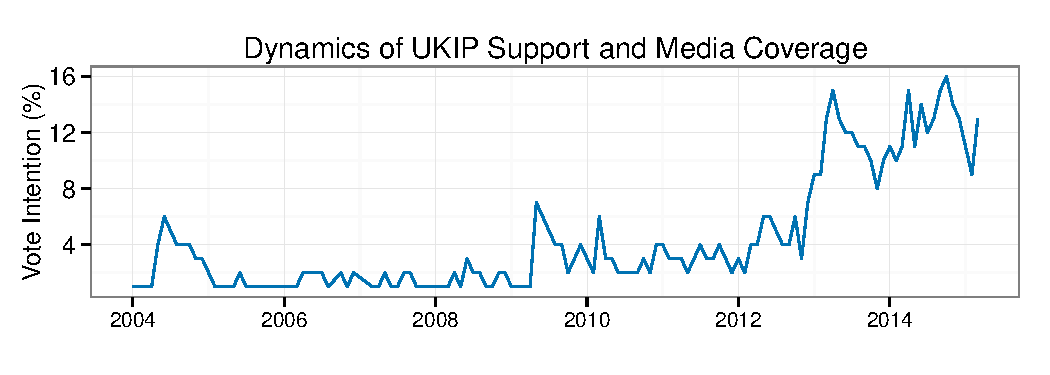
\includegraphics{ukip_media_files/figure-latex/unnamed-chunk-1-1.pdf}

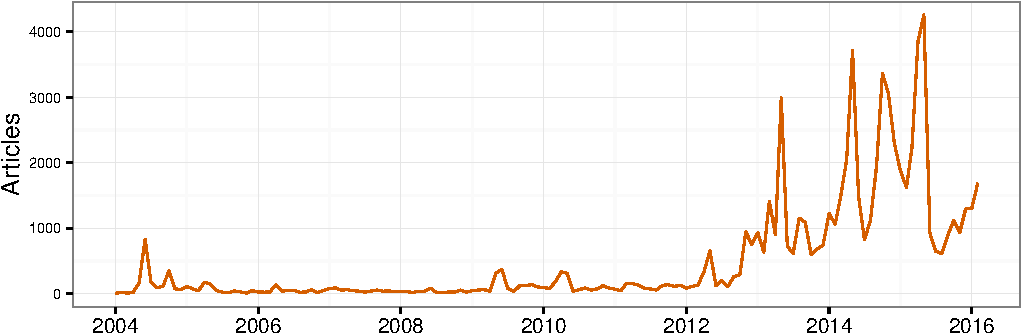
\includegraphics{ukip_media_files/figure-latex/unnamed-chunk-2-1.pdf}

\begin{figure}[htbp]
\centering
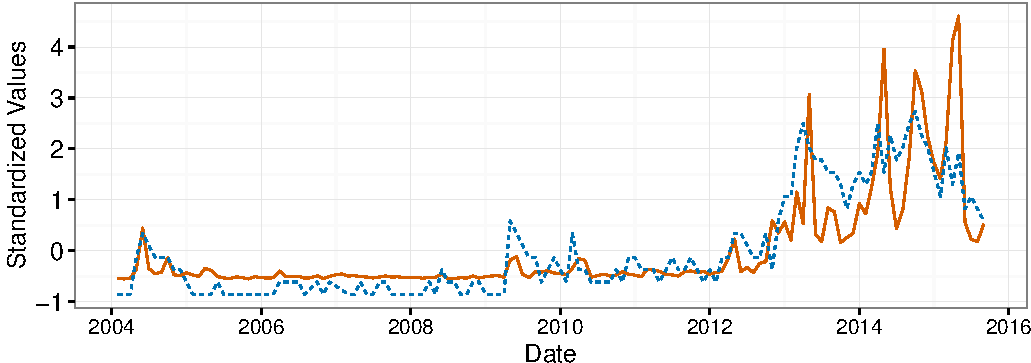
\includegraphics{ukip_media_files/figure-latex/unnamed-chunk-3-1.pdf}
\caption{Dynamics of UKIP Support and Media Coverage}
\end{figure}

\setlength\parindent{24pt}

The variable \emph{Articles} reflects the number of articles Nexi s
returns from the first day of each month until the last day of each
month. Figure 1 provides a summary view of the two main variables of
interest. The dotted line represents \emph{Support} and the solid line
represents \emph{Articles}. Raw values are displayed in the first two
(top) panels. For ease of direct comparison the bottom panel displays
standardized scores in which each value is derived by subtracting the
mean of the particular time-series and dividing by one standard
devation.

It is also plausible that elections have an independent effect on
coverage and support due to general increased media attention and
campaigning. For this reason, we have included eponymous dummy variables
for the months of each national and European election within the
sampling period. The elections included are three European elections
(June 2004, June 2009 and May 2014) and three general elections (May
2005, May 2010, and May 2015). European elections coincide with local
elections in the UK.

In the present analysis we do not consider public opinion on particular
political issues, measures of objective political or policy dynamics, or
the visibility of party leaders in the media, for several reasons. The
first and main reason is dictated by our problem-driven approach.
Because our contribution to the literature is motivated by a particular
debate in the politics of British media, we focus on the parameters of
that debate, which have revolved around party coverage. Although UKIP's
controversial leader Nigel Farage is likely a significant aspect of
UKIP's media visibility, coverage of Farage is almost certainly highly
correlated with coverage of the party, as Vliegenhart, Boomgaarden, and
Van Spanje find of party and leader coverage in multiple other Western
European countries. Second, Vliegenhart, Boomgaarden, and Van Spanje
also find that media coverage of parties is, overall, more relevant than
party leader as a predictor of party support
\citep[333]{vliegenthart_anti-immigrant_2012}. While it is possible that
phenomena such as objective immigration levels, media coverage of
immigration, and/or public opinion on immigration may affect both UKIP
party coverage and public support for UKIP, it is not theoretically
straightforward that they should affect one of our main variables more,
or sooner, than the other. Because we lack any particular theoretical
perspective on such possibilities, and there are many additional causal
factors which could arguably be included in this system, we refrain from
proliferating additional variables \citep{Achen:2006fp}.

We first use econometric techniques to test for, and distinguish the
ordering of, potential causal dynamics between media coverage and public
support for UKIP. An ideal approach to testing the presented hypotheses
is vector autoregression (VAR) with Granger causality tests
\citep{brandt2007multiple, vliegenthart_anti-immigrant_2012}.
Specifically, we estimate a VAR by OLS per equation, using the following
form:

\begin{equation}
 \label{eq:VAR}
   y_t = A_1 y_{t-1} + \dots + A_p y_{t-p} + D_t + u_t
\end{equation}

where \(y_t\) is a \(K \times 1\) vector of endogenous variables and
\(u_t\) is the error term. In our case the endogenous variables are
\emph{Support} and \emph{Articles}. The coefficient matrices \(A_1\),
\(\dots\), \(A_p\) are of dimension \(K \times K\). By convention \(p\)
denotes the ``order'' of the VAR, or the number of lags used. Typically
this is determined empirically, as we do below. In addition, \(D_t\)
refers to a vector of exogenous regressors. In our case the exogenous
regressors include a constant term, a trend term, the dummy variable for
UK General Election months, and the dummy variable for European election
months. We then use the conventional F-type Granger-causality test for
each of the two endogenous variables in the system. The vector of
endogenous variables \(y_t\) is divided into two vectors \(y_1t\) and
\(y_2t\) of dimensionality (\(K_1 \times 1\)) and (\(K_2 \times 1\))
with \(K = K_1 + K_2\) \citep{Pfaff:2008wk}. The null hypothesis is that
no lags of variable \(y_{1t}\) are significant in the equation for
variable \({y}_{2t}\). If \(\alpha_{21, i} = 0\) for \(i = 1\), \(2\),
\ldots{}, \(p\), we say that \(y_{1t}\) does not ``Granger-cause''
\(y_{2t}\).

Additionally, a brief qualitative historical analysis of the dynamics is
conducted to further probe any potential causal process(es). It is
arguably a blindspot of quantitative time-series research to neglect
inquiry into the subsantive historical processes corresponding to the
statistical properties of time-series data. In particular, the
substantive nature of the puzzle at hand requires the identification of
a historical narrative which would not necessarily follow from a
statistical fact such as Granger causality. Even with econometric
evidence suggesting an association in one direction or the other, it
would not necessarily follow that a substantively and historically
significant process has occurred in the particular and contingent
history behind the time-series. For instance, it could be the case that,
formally, media coverage Granger-causes public support \emph{and} that
exogenous increases in media coverage have played no particularly
important role in the rise of UKIP support. This is because statistical
properties of time-series in no way preclude the fact that the
historically key moments of UKIP's rise could have been random or
contingent consequences of other factors. Also, it is always possible in
any particular historical process that \(Y_1\) has an average effect on
\(Y_2\) which is statistically significant but in key, contingent
moments certain shifts in \(Y_2\) may explain unique changes in \(Y_1\)
in a fashion which happens not to be statistically distinguishable. In
the latter case, media-caused increases in public support might
themselves be responding to, and amplifying, contingent but exogenous
increases in public support in an arguably democracy-consistent fashion,
even if increases in support do not statistically predict increases in
media coverage.

To provide the strongest possible investigation of a possibly dynamic
relationship between media coverage and UKIP support, we will need to
assess the degree to which increases in media coverage have been
followed by increases in public support for UKIP following
\emph{stagnant or decreasing} levels of support in preceding months. We
will then also need to assess the degree to which such identifiable
historical moments were related to the relatively few key moments in
which support for UKIP rises most dramatically. We explore these
substantive questions with a brief narrative of the political events and
media topics which lie behind our time-series data.

\section{Findings and Discussion}\label{findings-and-discussion}

Because both variables are non-stationary, vector autoregression is
estimated with first differences of each variable. Optimal lag length is
determined by the Aikeke Information Criterion to be VAR(3). The model
includes a constant and a trend term. Diagnostics suggest that using the
log of each variable before differencing reduces heteroskedasticity and
serial correlation of errors. The models displayed here all pass the
standard ARCH-LM and Portmanteau tests for non-constant error variance
and serial correlation of errors, respectively. Finally, diagnostics
show no evidence of significant temporal instability (see Supplementary
Information).

\begin{table}[!htbp] \centering 
  \caption{Vector Autoregression} 
  \label{} 
\begin{tabular}{@{\extracolsep{5pt}}lcc} 
\\[-1.8ex]\hline 
\hline \\[-1.8ex] 
 & \multicolumn{2}{c}{\textit{Dependent variable:}} \\ 
\cline{2-3} 
\\[-1.8ex] & \multicolumn{2}{c}{} \\ 
 & $\Delta Support$ & $\Delta Articles$ \\ 
\\[-1.8ex] & (1) & (2)\\ 
\hline \\[-1.8ex] 
 $\Delta Articles_{t-1}$ & 0.100$^{*}$ & $-$0.380$^{***}$ \\ 
  & (0.054) & (0.092) \\ 
  & & \\ 
 $\Delta Support_{t-1}$ & $-$0.500$^{***}$ & $-$0.025 \\ 
  & (0.100) & (0.180) \\ 
  & & \\ 
 $\Delta Articles_{t-2}$ & 0.091$^{*}$ & $-$0.340$^{***}$ \\ 
  & (0.053) & (0.091) \\ 
  & & \\ 
 $\Delta Support_{t-2}$ & $-$0.260$^{**}$ & $-$0.140 \\ 
  & (0.100) & (0.170) \\ 
  & & \\ 
 $\Delta Articles_{t-3}$ & 0.091$^{*}$ & $-$0.190$^{**}$ \\ 
  & (0.052) & (0.089) \\ 
  & & \\ 
 $\Delta Support_{t-3}$ & $-$0.110 & $-$0.160 \\ 
  & (0.095) & (0.160) \\ 
  & & \\ 
 Constant & 0.004 & 0.026 \\ 
  & (0.070) & (0.120) \\ 
  & & \\ 
 Trend & 0.0001 & 0.0001 \\ 
  & (0.001) & (0.001) \\ 
  & & \\ 
 General Elections & $-$0.098 & 0.270 \\ 
  & (0.240) & (0.420) \\ 
  & & \\ 
 EU Elections & 0.430 & 1.400$^{***}$ \\ 
  & (0.260) & (0.450) \\ 
  & & \\ 
\hline \\[-1.8ex] 
Observations & 142 & 142 \\ 
R$^{2}$ & 0.150 & 0.230 \\ 
Adjusted R$^{2}$ & 0.097 & 0.180 \\ 
Residual Std. Error (df = 132) & 0.400 & 0.680 \\ 
F Statistic (df = 9; 132) & 2.700$^{***}$ & 4.400$^{***}$ \\ 
\hline 
\hline \\[-1.8ex] 
\textit{Note:}  & \multicolumn{2}{r}{$^{*}$p$<$0.1; $^{**}$p$<$0.05; $^{***}$p$<$0.01} \\ 
\end{tabular} 
\end{table}

Initial VAR results show little evidence that changes in public support
predict media coverage, but statistically significant evidence that
media coverage drives public support. As the numerical results in Table
1 show, there is no statistically discernable correlation between past
changes in public support and changes in media coverage, whereas past
changes in media coverage have a statistically significant correlation
with future changes in public support, as the coefficients for each
distributed lag of \(\Delta Articles\) in Equation 1 are positive and
significant. As reported in Table 2, Granger causality tests also
support H1 that changes in media coverage are associated with future
changes in public support while they do not support the reverse
relationship hypothesized in H2, as the true coefficients for the lags
of \(\Delta Articles\) in Equation 1 are very unlikely to all be zero
(p=.054) while we fail to reject the possibility that all of the
coefficients for \(\Delta Support\) in Equation 2 are zero (p=.74).

Because our endogenous variables are first differences of the natural
logarithm, the coefficients in Table 1 can be interpreted as
elasticities. That is, the coefficients in Equation 1 and Equation 2 are
approximations of the expected growth rate in \(Y_2\) associated with a
one percent increase in \(Y_1\) at each of its lagged values. To gain a
sense of how \emph{Support} responds to \emph{Articles}, the typical
approach is to use impulse response functions, which trace the effect of
a random one-unit shock in one variable on future values of a second
variable in the system.

In Figure 2 and Figure 3, we generate orthogonalized impulse response
plots. We consider orthogonalized or uncorrelated shocks because we are
most interested in what happens when one variable changes for reasons
that do not also lead to changes in the other variable. The x-axis
reflects time periods following on an initial shock in the error term of
one variable, while the y-axis reflects the expected changes in the
other variable.

\begin{table}[!htbp] \centering 
  \caption{Granger Causality Tests} 
  \label{} 
\begin{tabular}{@{\extracolsep{5pt}} ccc} 
\\[-1.8ex]\hline \\[-1.8ex] 
 & Support & Articles \\ 
\hline \\[-1.8ex] 
P-value & $0.054$ & $0.740$ \\ 
DF1 & $3$ & $3$ \\ 
DF2 & $264$ & $264$ \\ 
F-test & $2.600$ & $0.410$ \\ 
\hline \\[-1.8ex] 
\end{tabular} 
\end{table}

\begin{figure}[htbp]
\centering
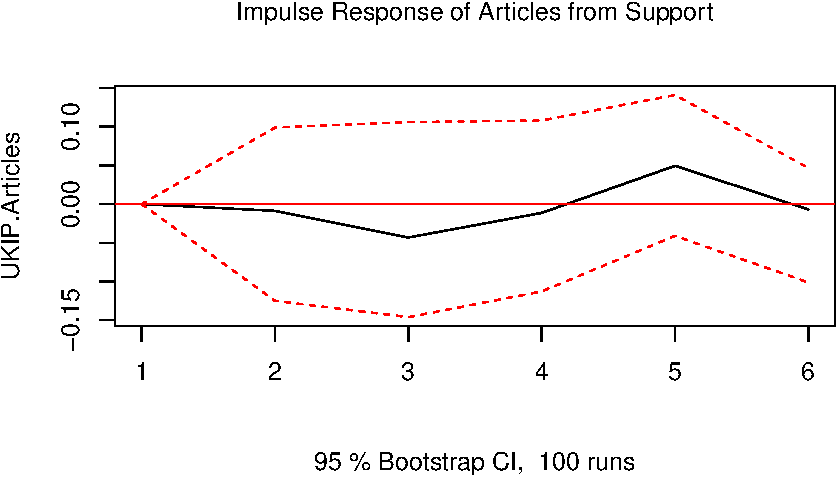
\includegraphics{ukip_media_files/figure-latex/unnamed-chunk-7-1.pdf}
\caption{Impulse Response Plot Shows Effect on Articles from an
Exogenous Increase in Support}
\end{figure}

\begin{figure}[htbp]
\centering
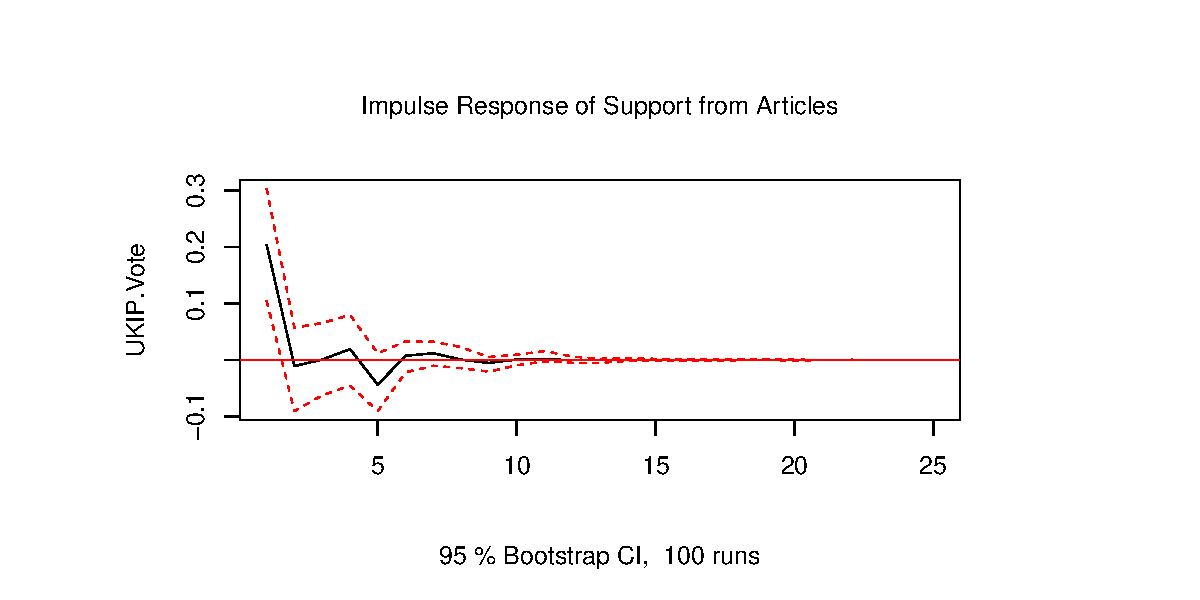
\includegraphics{ukip_media_files/figure-latex/unnamed-chunk-8-1.pdf}
\caption{Impulse Response Plot Shows Effect on Support from an Exogenous
Increase in Articles}
\end{figure}

To interpret the estimated effect media coverage has on UKIP support,
consider the impulse response function plotted in Figure 3. The maximum
number of monthly articles observed in the sample is 4256, therefore a
one-percent increase in articles is equal to a monthly increase of about
43 articles. The maximum value of \emph{Support} is 16, so the first
period of the impulse response (0.19) suggests that in response to a
43-article increase, \emph{Support} would increase by about 19\% of 1\%
of 16\%. This amounts to an increase of roughly 0.03\% of the population
reporting an intention to vote for UKIP. While this hypothetical effect
of a small increase in coverage is minute, the history of UKIP's media
coverage contains several months of exceptionally large increases in
reporting. Those months in the top 1\% of article growth (the 99th
percentile) were characterized by article growth of 1649 articles or
greater, that is, a growth rate of 38.75\% or greater. By the preceding
calculations, a 38.75\% increase in articles would be associated with a
7.25\% growth rate in \emph{Support}, equivalent to a 1.16-point
increase in the percentage of the population reporting an intention to
vote for UKIP.

Finally, with respect to the statistical modeling, we note there are
limitations of the data which may make it difficult to identify the full
range of causal effects in a VAR approach. First, it is possible that
monthly measures are too infrequent to capture causal effects if the
real lag between effects is shorter than one month. Also, importantly,
structural tests on all models suggest strong evidence of instantaneous
causality. Thus, the VAR results suggest clear but imperfect and, for
reasons discussed above, inherently limited evidence for Hypothesis 1
that increases in media coverage lead to increases in public support.
The VAR results provide no evidence for Hypothesis 2, that increases in
public support lead to increases in media coverage. Given the problem of
instantaneous causality, we cannot rule out the possibility that both
variables drive each other in periods shorter than one month or that
both variables are driven by some third unobserved variable.
Nonetheless, an empirical fact of our data is that media coverage
Granger-causes public support and not vice-versa.

\section{Qualitative Analysis}\label{qualitative-analysis}

To what extent are the statistical regularities identified by the vector
autoregression historically significant causal factors in the rise of
public support for UKIP? To facilitate a qualitative investigation of
the dynamics, we quantitatively identified months which meet criteria
similar to the concept of Granger causality. Any month (\(t\)) that is
immediately preceded by two months (\(t-1\), \(t-2\)) of stagnating or
declining public support but increased media coverage, we designate as a
month of ``uncaused'' media increase or media ``bias'' for short.
Symmetrically, any month that is immediately preceded by two months of
stagnating or declining media coverage but increasing public support, we
consider a month of ``uncaused'' or exogenously increasing public
support. To mitigate the probability we will be counting mere noise as
meaningful increases, we count as increases only those greater than .05
standard deviations and all other months as ``stagnating or
decreasing.'' Figure 4 presents the standardized values of each time
series with dot-dash vertical lines indicating months of uncaused media
`bias' and long-dash vertical lines indicating months of uncaused
increases in public support. A first consideration of Figure 4 reveals
that increases in media coverage unwarranted by public support are not
only roughly as frequent as uncaused increases in public support, but
they are found at multiple pivotal months in periods of the most
dramatic increases in UKIP's public support. To be clear, we are not
claiming to pinpoint key moments of causal effect; in any particular
point of the time-series, it is impossible to know whether a particular
pattern represents a random or systematic component. Rather, we take the
evidence from the VAR to be our warrant for exploring the qualitative
data in search of examples whereby the substantive significance of the
statistical evidence may either be better illustrated or possibly
discounted due to untheorized contingencies. Based on Figure 4, we focus
especially on two key periods: from July to September of 2012, and the
second half of 2013.

UKIP, formed in 1993, began fielding European parliamentary candidates
in 1994 and British parliamentary candidates in 1997. Since then, the
party has enjoyed mixed but notable increases in public support and in
electoral outcomes, particularly in the European parliament where the
party was the largest in the 2014 election. Until the 2015 general
election, UKIP's domestic electoral success had been much less
impressive, receiving just 3.1\% of the vote in 2010. Like other small
or new parties, it has a history of infighting, changes of direction and
leadership, and problems with financial mismanagement
\citep{Whitaker:2011gi}. As recently as 2011, a lack of media attention
was cited as a factor in UKIP's poor performance, as well as credibility
and relatively few activists \citep{ford_strategic_2012}. Indeed, the
historical pattern of both media coverage and public support for UKIP
over much of its recent history, from 2004 to 2009, was a series of
small increases which consistently returned to low baseline quantities
of little political consequences.

The party experienced its first increases in both coverage and voting
intention in 2004 with the European election, in which they received
16\% of the vote, where coverage reached 829 articles in a single month,
their record amount of coverage at the time and the greatest amount of
coverage the party would experience until 2012. During this spike, both
media coverage and voting intention increase proportionately and as
would be expected if coverage was driven by public opinion: Figure 4
indicates no media bias or exogenous increases of support in this
instance. Following this, both coverage and support decay and return to
poltically negligible levels. Over the next eight years, there are a
range of events that do not attract very much media attention or public
support; indeed, events occur between these years that are similar to
those that will occur in later years but they fail to generate the
extraordinary media attention gained by such events in later years. The
vast majority of coverage refers to everyday factual information such as
reports of election results, or else it tends to report claims of fraud
and infighting. Indeed, Figure 4 shows that this period was
characterised by several small, quickly decaying increases in support
not predicted by media coverage, consistent with the claim that a lack
of media coverage failed to facilitate public support through this
period \citep{ford_strategic_2012}.

Apart from the 2005 election, in which UKIP received little coverage and
performed poorly (receiving just 149 articles in that month)
\citep{election_2005, morris_election_2005}, UKIP saw little change in
public support or media coverage until the European elections of 2009.
There is a small boost in both support and coverage in April 2006, when
David Cameron calls the party `fruitcakes, loonies' and `closet racists'
\citep{white_ukip_2006}. Interestingly, this rise in media coverage was
followed by a small but sustained boost in public support, which
persisted for three months. In April 2008, Conservative MP Bob Spink
defected, giving UKIP their first MP which generated very little
coverage, despite being called a coup \citep{winnett_tory_2008}. Even
the European election in 2009, in which UKIP came in second place,
generated far less coverage than the 2004 European election, where the
party came in third place (829 to 320 articles in a month,
respectively). Despite this, it was still hailed as a `political
earthquake' \citep{watt_european_2009} and garnered coverage for UKIP's
leader Nigel Farage.

\begin{figure}[htbp]
\centering
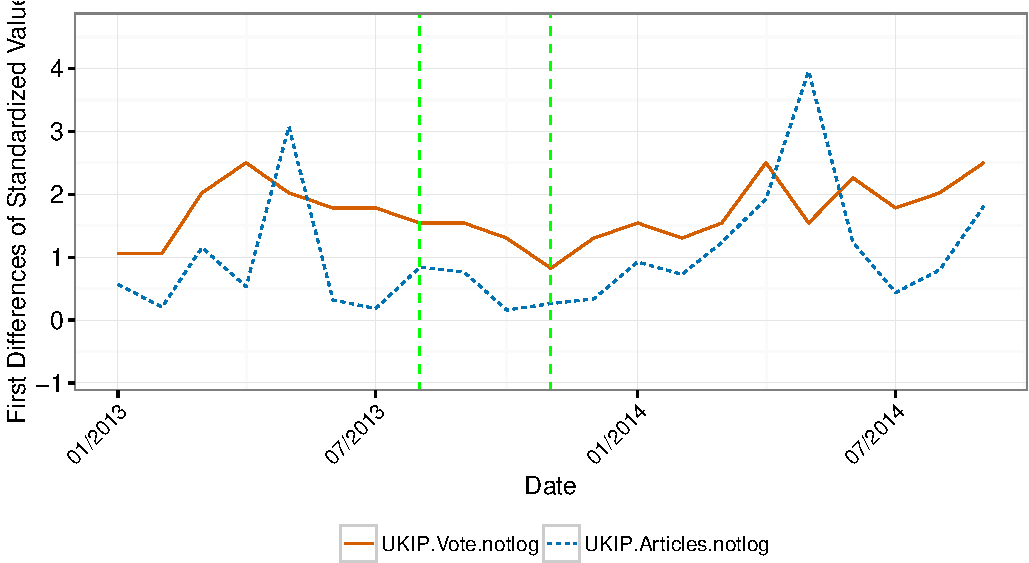
\includegraphics{ukip_media_files/figure-latex/unnamed-chunk-9-1.pdf}
\caption{Standardized Time-Series, Green Dot-Dash Lines Indicate Media
``Bias'' and Yellow Long-Dash Lines Indicate Exogenous Increases in
Support}
\end{figure}

Following this, there are at least two sets of months in which increased
media coverage is not caused by changes in UKIP's public support but is
followed by some of UKIP's most historically crucial increases in public
support. Using Figure 4 as a guide, we consider in greater detail the
two months of ``uncaused'' increases in coverage near the middle of 2012
(July and September) and the second half of 2014 (August and November).
Readers may refer to Supplementary Information for an additional plot
that magnifies this particular section of Figure 4. This period includes
three by-elections (Corby, Middlesborough and Rotherham), with many
being controversial \citep{wainwright_rotherham_2012}, as well as the
UKIP party conference. All three of these by-elections occurred in
November 2012; UKIP placed second in two and third in Corby, with the
Rotherham by-election's 21\% vote share being the party's highest up to
that point. In July 2012 UKIP's public support was unremarkably near its
average and was declining from June, after it had been stagnant since
May. But media coverage held relatively steady, slightly decreasing once
but slightly increasing twice (and slightly increasing overall) from
June to September, from 123 to 261 articles. It is only at this point
that public support increases notably from September to October and is
followed by a spike in media coverage that likely represented a moment
of positive feedback ending in the first truly significant rise of UKIP
into mainstream public consciousness - up to 15\% support in April 2013.

Between August and November 2012, the amount of articles covering UKIP
increased from 198 to 948, the most they had ever received in one month
at the time, beyond three standard deviations from their long-term mean.
To be clear, this dramatic surge of UKIP support appears to launch with
a moment of postive feedback betwen support and media coverage,
beginning with a notable spike in public support. However, the months of
July and September 2012 are months in which media coverage is slightly
increasing despite stagnant or declining levels of public support, and
it is these dynamically unresponsive months of media coverage that
precede the spike in support observed in October. Of course, it is
impossible to distinguish these slight increases in media coverage in
July and September from random noise in the polling; but from the
statistical analysis we have reason to believe such moments of
unresponsively increasing media coverage are at least comparatively more
likely to be predictve of changes in support than vice versa. Thus,
while it would be impossible to demonstrate conclusively that these
months of media coverage played a causal role in the dramatic rise of
support achieved by November, our model suggests it is more likely these
unresponsively stable and slightly increasing months of media coverage
played a causal role in the increased support of October, than it is
that the increased support in October played a causal role in the
then-highest level of media coverage seen in November. In turn, the
unprecedently high levels of media coverage in November likely played
more of a role in the following spike of support than the October spike
in support played in the November spike in media coverage. This
interpretation is enhanced by the additional fact that after the spike
in support of October, November returned to the lowest level of support
observed in several months. Again, while we cannot confidently read
causal dynamics in particular data points, the point is that the
increase in support of October, which ostensibly seems to be followed by
a spike in media coverage ultimately leading to UKIP's real debut, is a
less plausible interpretation of the data than one based on Hypothesis
1.

Now consider the period between July 2013 and December 2014. Despite
public support declining rapidly and steadily from its high point in
April 2013, media coverage from July to August increases considerably,
from 613 to 1154 articles in the month. Public support continues to
decline through August until November, decreasing from 11\% to 8\%.
While media coverage appears to adjust dynamically downward after its
``uncaused'' increase of August, yet again in November media coverage
stabilizes and slightly increases. It is only at this point in November
that support ends its long and steady decline and yet again begins
another substantial increase until it returns back to the high levels of
April 2013. Again, in these two months we identify apparently minor but
potentially crucial non-dynamically-responsive levels of media coverage
which may be functioning as a floor preventing support from continuing
to decline and making possible the surge beginning from November 2013.
While of course these spikes and drops in support may just be volatility
around UKIP's new, higher mean levels of support, the key point here is
only to explore and give possible instances of the statistical findings.
Unlike the previous instance of ``bias'' explored above, where political
events such as by-elections and the party conference season may have
played roles, in this case there are no obvious and directly
party-related events shaping the dynamics in this period. However, one
key event which may have played a role at this time is the lifting of
work restrictions on Romanian and Bulgarian nationals which occurred in
January 2014 \citep{martin_immigration_2013}, with media coverage
intensifying in the months leading up to January. The increased salience
of issues related to migration and the European Union may help to
explain changes in media coverage independent of UKIP's support.
Interestingly, considerable coverage also surrounded Farage's comment,
in December 2013, that Britain should accept Syrian refugees
\citep{goodman_does_2013}.

Previous studies have relied on statistical models similar to the one we
have presented here. However, a qualitative appreciation of the data
indicates at least two key examples where increased media coverage
unwarranted by changes in public support take place in key periods of
UKIP's rise.

\section{Conclusion}\label{conclusion}

This study has made three contributions. First, to our knowledge this is
one of the first articles to study the dynamics of right-wing populist
party support and quantity of media coverage in the context of a
majoritarian system and the UK in particular; previous research has
primarily focused on other West European democracies such as Belgium,
the Netherlands and Germany. Despite the change in political system,
this study has shown quantitative and qualitative evidence that media
coverage may have played a unique causal role in increasing support for
UKIP, in a fashion irreducible to previous levels of support or election
outcomes.

Second, these findings are of significance to contemporary public debate
in the UK concerning the perception that unfair quantities of media
coverage are given to UKIP. Some have argued that extensive media
coverage of UKIP is justified due to public support for the party. The
findings here, on the other hand, are inconsistent with this argument:
the extraordinary media coverage which has been given to UKIP cannot be
explained or defended on grounds of public support. We find that media
coverage has no reliable relationship to public support in the one
month, two months, or three months before a particular month of
coverage. Indeed, we find that coverage may have independently and
uniquely driven some of the very public support which media regulators
would later point to as their justification for the extraordinary
coverage given to UKIP. Our findings therefore raise serious questions
for the function of media coverage in a democratic political system,
because they suggest that unelected and unrepresentative actors (the
media) may be systematically shaping public opinion toward, and the
fortunes of, certain political parties in contradiction to organic
levels of public support for those parties.

Third, this article contributes to currently on-going efforts to advance
the methodological aspects of research on media and public opinion
\citep{Vliegenthart:2014di}. Unlike many quantitative studies, we
provide an analytically sophisticated qualitative investigation of our
statistical findings. Most previous research on the visibility-support
nexus relies primarily on statistical evidence, which cannot necessarily
address important questions relating to the substantive historical
narrative of a particular political party. We find that, in two periods,
increases in media coverage came after two months of stagnating or
declining public support but was then followed by historically pivotal
increases in support. While we cannot claim these periods are definitive
instances of causality, they show that the particular and contingent
historical unfolding of UKIP is consistent with the inference, suggested
by our statistical analysis, that media coverage played a unique and
important causal role in the rise of public support for UKIP.

\newpage

\section{Supplementary Information}\label{supplementary-information}

\begin{figure}[htbp]
\centering
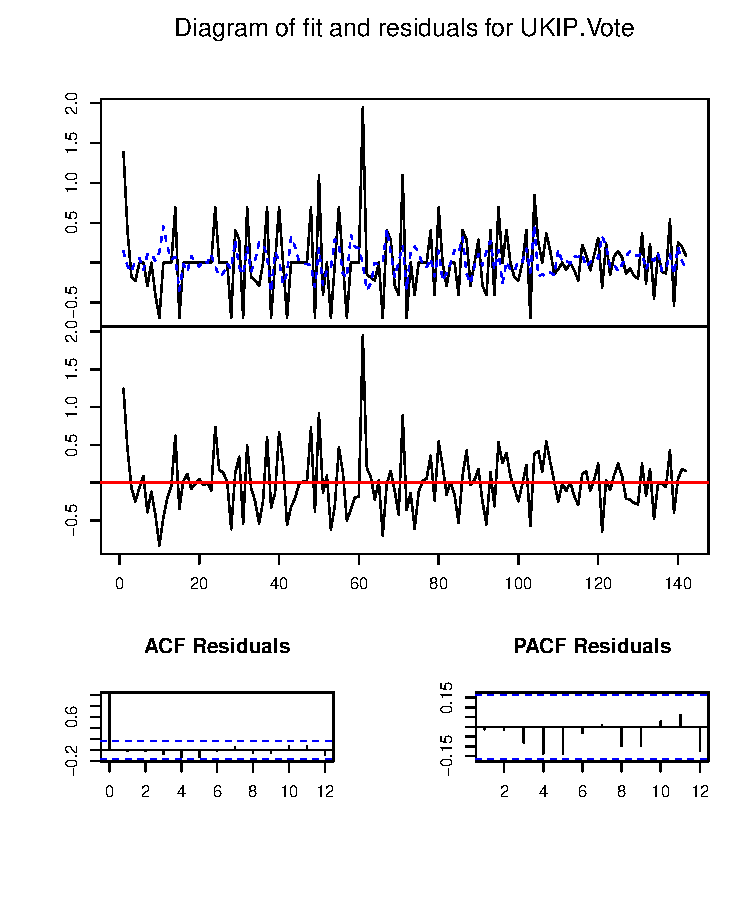
\includegraphics{ukip_media_files/var-plot-support.pdf}
\caption{VAR Diagnostics for Support}
\end{figure}

\pagebreak

\begin{figure}[htbp]
\centering
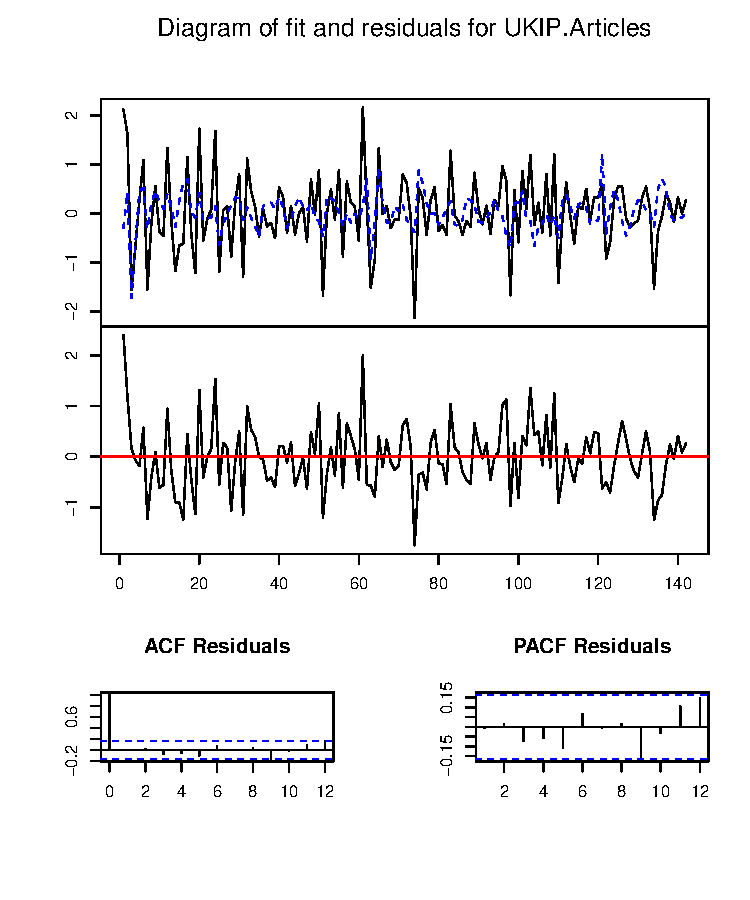
\includegraphics{ukip_media_files/var-plot-articles.pdf}
\caption{VAR Diagnostics for Articles}
\end{figure}

\pagebreak

\begin{figure}[htbp]
\centering
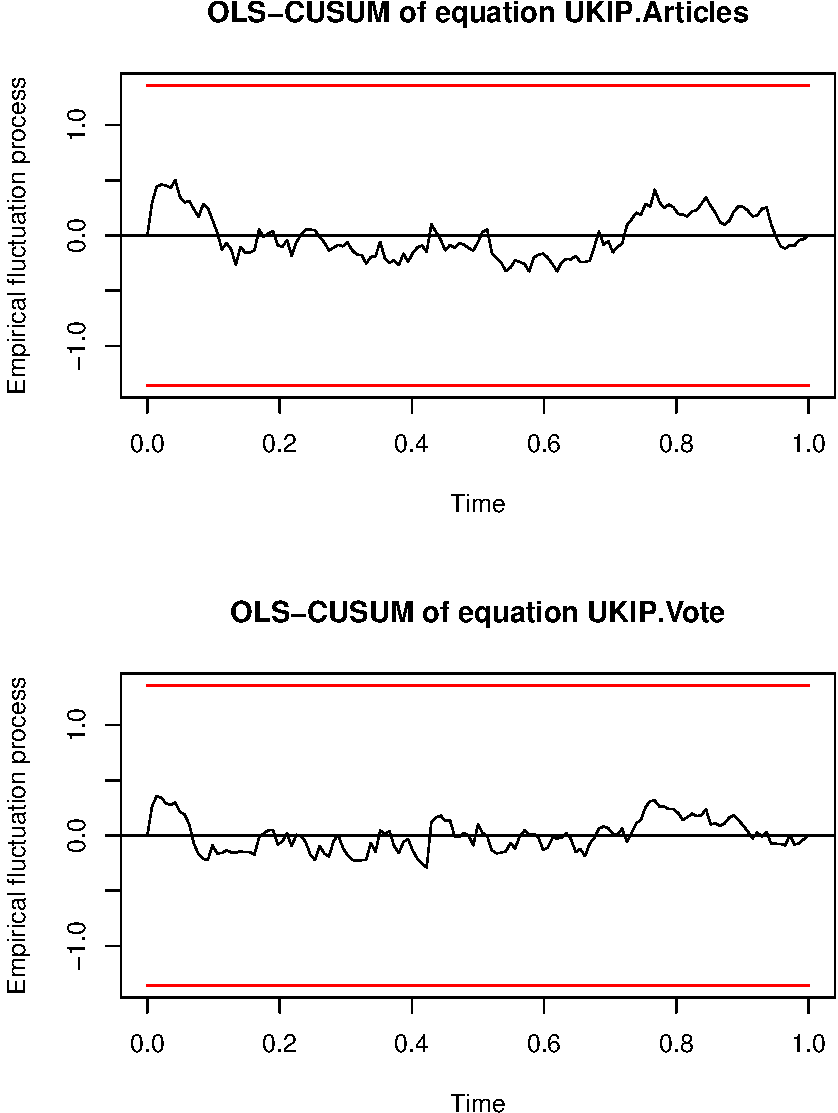
\includegraphics{ukip_media_files/figure-latex/stability-check-vote-1.pdf}
\caption{Checking temporal stability of VAR model with cumulative sums
of residuals}
\end{figure}

\newpage

\subsection{Breusch-Godrey Test of serially correlated errors for VAR
model}\label{breusch-godrey-test-of-serially-correlated-errors-for-var-model}

\begin{verbatim}
## 
##  Breusch-Godfrey LM test
## 
## data:  Residuals of VAR object varmodel
## Chi-squared = 20, df = 20, p-value = 0.2
\end{verbatim}

\subsection{Multivariate ARCH-LM test for heteroskedasticity in Var
model}\label{multivariate-arch-lm-test-for-heteroskedasticity-in-var-model}

\begin{verbatim}
## 
##  ARCH (multivariate)
## 
## data:  Residuals of VAR object varmodel
## Chi-squared = 40, df = 40, p-value = 0.8
\end{verbatim}

\newpage

\begin{figure}[htbp]
\centering
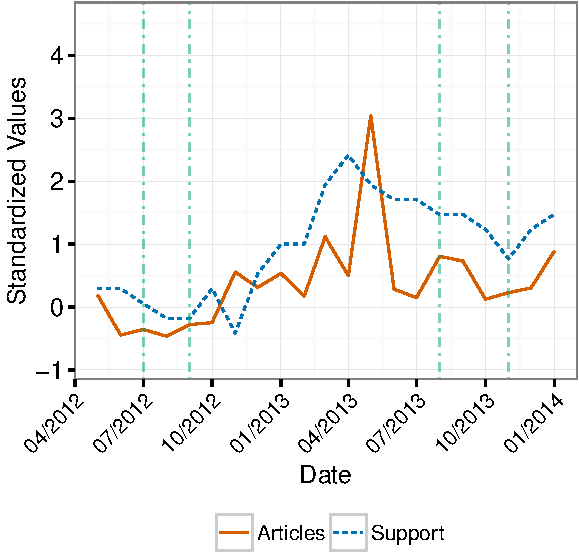
\includegraphics{ukip_media_files/figure-latex/qual-zoomed-plot-1.pdf}
\caption{Standardized Time-Series with Green Dot-Dash Lines Indicating
Non-Responsively Increasing Media Coverage, April 2012 to January 2014}
\end{figure}

\newpage

\bibliography{mybib}

\end{document}
